\chapter{Speed} \label{chap:speed}


% bottlenecks induced by FLOPs oriented optimizations - говорю о том, что определине "маленькая" сеть и "быстрая" сеть неоднозначны. можно смотреть на параметры, можно на FLOPS, можно на MAC, можно на real-life performance. ссылаюсь на работы которые показывают что связь между FLOPS | params | mac и скоростью нифига не линейная. можно вставить графики сравения по FLOPS похожие на те что в \cite{ma2018shufflenetv2}

\section{Introduction}

% сложно разделить скорость и качество, кпотому что часто новые блоки которые быстрее, одновременно дают еще и более хорошее качество. Цель это главы скорее в другом - понять от чего зависит скорость конкретных блоков (memory bound) и почему некоторые слои лучше не использовать. Эта глава закладывает фундамент для дизайна более хорошей сетки в следующих главах


Real world tasks often have computational constrains on the design of architectures. Design of light-weight models with good speed-accuracy tradeoffs has been explored extensively before \cite{howard2017_mobilenetv1} \cite{sandler2018_mobilenetv2} \cite{ma2018_shufflenetv2} \cite{zhang2018_shufflenet}.  % \cite{Xception} 

To measure complexity of the model some works use number of computations it does. Examples of such metrics are floating point operations (FLOPs) and multiply-accumulate operations (MACCs). Other focus on minimizing of number of trainable parameters. This metrics are indirect approximation of direct metric such as speed or latency. Previous works has shown \cite{radosavovic2020_designing} \cite{lee2020_compounding_improvements} that factors affecting inference latency on modern accelerators are complicated and direct measurement on target device should be preferred. This phenomenon is illustrated on \autoref{fig:fps_from_params}, which shows that speed doesn't correlate with number of model parameters.   
% TODO actually draw this figure

\begin{wrapfigure}{r}{0.25\textwidth} %this figure will be at the right
    \centering
    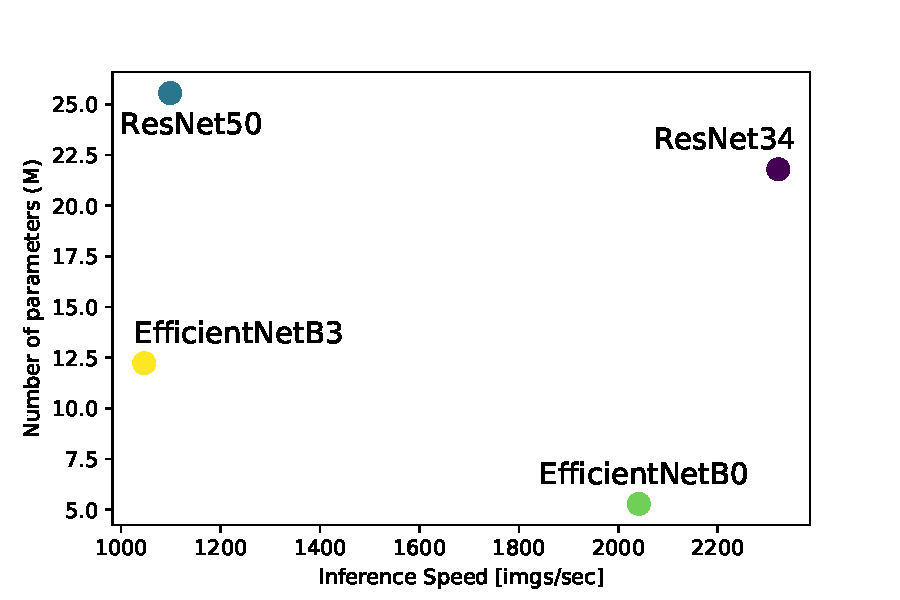
\includegraphics[width=0.26\textwidth]{images/fps_from_params.pdf}
    \caption{Inference speed vs Number of parameters for several classification models. It can be seen that they speed have very low correlation with number of parameters and thus FLOPs.}   \label{fig:fps_from_params}
\end{wrapfigure}

The goal of this chapter is to explore bottlenecks induced by FLOPs oriented optimizations and show that taking into consideration limitations of current accelerators could help to develop guidelines for architecture design which do not compromise speed. We first explore the memory-bound problem theoretically, then prove out reasoning with experiments on current GPU accelerators, and finally come up with simple principles to follow. 

The deep learning models could be run on CPU or on a number of other accelerators. Most popular ones being GPUs (graphic processing units) and TPUs (Tensor processing units). 
%, ... (тут примеры других ускорителей). (тут статистика по использованию акслелераторов)
This works focuses on optimizing and developing networks specially optimized for \textbf{modern GPUs}, such narrow focus allows to better utilize the knowledge about what constrains speed the most. Obtained results may not be applicable if models have to be run on CPUs or mobile devices. % (тут можно что-то из Effnet lite процитировать). 



% \cite In-datacenter performance analysis of tensor processing units
% \cite The deep learning revolution and its implication for computer architecture and chop desin

\section{Definitions}

"It’s dot products all the way down" 

Many of the computations inside neural networks are dot products like this: $y = w[0]*x[0] + w[1]*x[1] + \ldots + w[n] * x[n]$ where $w$ and $x$ are two vectors and $y$ is a scalar. There are two main ways to calculate number of computations in such operation. First is to count $ w[0] * x[0] + \ldots $ as single multiply-accumulate or 1 \textbf{MACC}. The \textit{accumulation} operation here is addition. In the example above we have $n$ MACCs. \footnote{Technically speaking there are only n - 1 additions in the example above. Think of MACCs as being an approximation, similar to Big-O notation used in approximation of algorithm complexity.}

Second is to count number of direct floating point operations (\textbf{FLOPs}), in the example above there are $2n - 1$ FLOPs, since there are n multiplications and n additions. FLOPs should not be confused with floating point operations per second (FLOPS) used to measure hardware performance. Because matrix-multiplications is the core operation in neural networks, many modern accelerators have special multiply-and-accumulate units, called tensor cores 
% \cite Volte: performance and programmability 
in GPUs and matrix multiply units in TPUs % \cite two papers from comments above [30] [14] in Searching ....
This means that 1 MACC could be performed using 1 instruction, so in this work definition of FLOPs follows \cite{zhang2018_shufflenet}, i.e. number of multiply-adds. Making FLOPs and MACC interchangeable.

Another important property of the network is dynamic random-access memory (\textbf{DRAM}) traffic for read and write of model parameters, activations and intermediate feature maps. Measuring exact number of DRAM read/write bytes could be complicated and requires special software. DRAM could be approximated by memory footprints of input and output tensors plus memory required for storing weights. This metric is called Convolutional Input/Output (CIO) \cite{chao2019_hardnet} and is proportional to to the real DRAM traffic measurement. For a typical convolution $K \times K$ kernel with $C$ channels, width $W$ and height $H$, CIO could be calculated using eq \ref{eq: CIO}
% TODO rewrite formula and add weighs term

\begin{equation}
    C I O=\sum_{l}\left(C_{in}^{(l)} \times w_{in}^{(l)} \times h_{in}^{(l)}+c_{o u t}^{(l)} \times w_{o u t}^{(l)} \times h_{o u t}^{(l)}\right)
    \label{eq: CIO}
\end{equation}

\section{Why FLOPs and latency do not correlate}


% (воткну сюда, потом разберусь в compounding тоже говорил что не наблюдают связи между FLOPS и скоростью. может надо воткнуть это как рефернс куда-то)
%% TODO: maybe need to move MoC into definition??
%% TODO: also later I use a slightly different MoC which also accounts for number of parameters accesses. Need to modify definition here, or use true MoC in later chapter
%% TODO: this chapter could be expanded by elaborating more on roofline analysis. could replot figures from \cite{li2021_searching}


We reasonably assume that model speed is either compute-bound or memory-(bandwidth)-bound as they don't fit in on-chip memories. DRAM access can dominate system inference time due to limited memory bandwidth. An ML model can achieve peak FLOPs/sec and fully utilize accelerators only when its operational density, which is MACs over CIO (MoC) is sufficiently large (and is enough to saturate accelerators performance (?? need to clarify \textit{saturate} ). 
From that we can see why minimizing number of FLOPs don't always correlate with latency, such minimization is only reasonable when we are compute-bounded in this layer. 

Several papers has observed this lack of correlation and proposed several key principles for designing high speed models specifically on GPUs \cite{radosavovic2020_designing} \cite{lee2020_compounding_improvements}. Rather than providing them as is we will validate each claim with a set of experiments to observe the switch between compute-bound/memory-bound regions directly for different type of layers.

\subsection{Depthwise Separable Convolutions}

Depth-wise convolutions (DW conv in short) have been proposed as an efficient alternative to traditional 2d convolutions. In the regular 2d convolution the filter is as deep as the input and lets us freely mix channels to generate each element in the output. In Depthwise convolution each channel is kept separate. 

Mixing channels is important for  neural networks, so the depthwise is more commonly used in combination with an additional step to mix the channels (pointwise convolution), such operation is called depthwise-separable convolution (DepSep conv in short). See \ref{fig: convs} for visual explanation of difference between conv and DepSep conv. 

\begin{figure}[h]
    \centering
         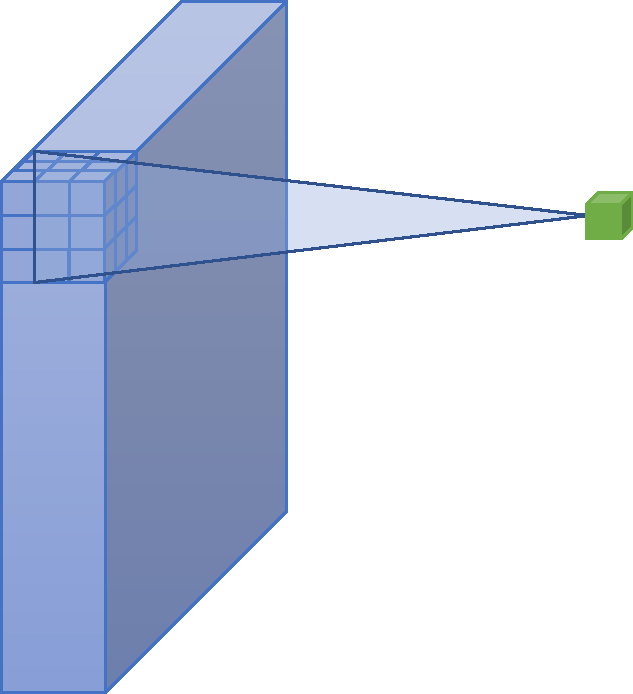
\includegraphics[width=0.26\textwidth]{images/conv.pdf}
         \hfil
         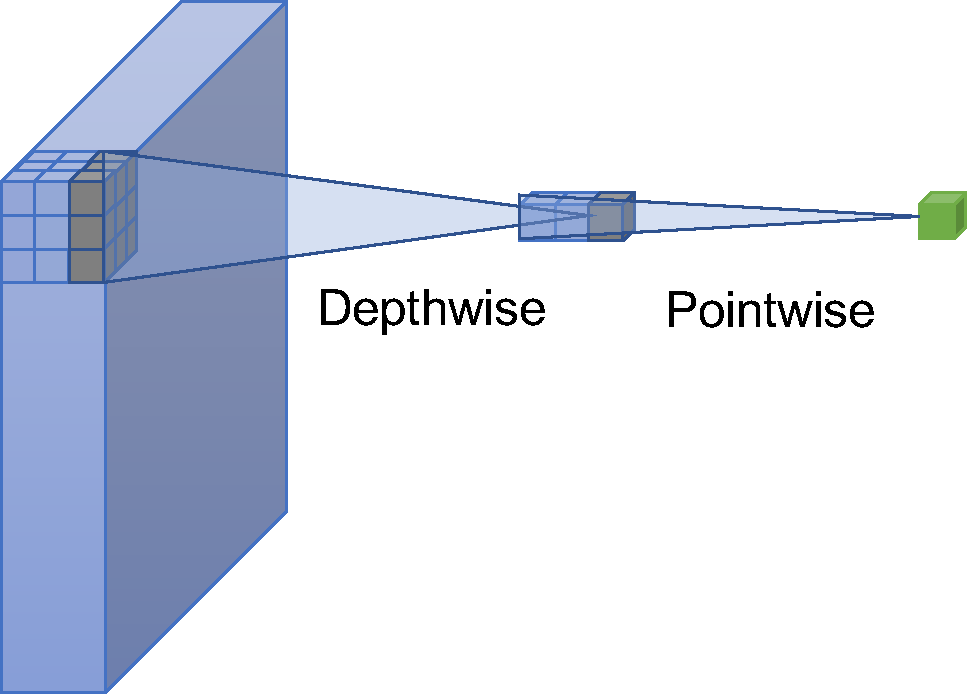
\includegraphics[width=0.4\textwidth]{images/conv_DepSep.pdf}
    \caption{Standard convolution and depthwise separable convolution.}   \label{fig: convs}
    \end{figure}


DepSep convolutions are used in models such as (cite excpetion mobilenet effnet) and more. They have less parameters and require less floating point operations (FLOPs) to compute, however as we mentioned above metrics such as FLOPs and parameter sizes may not correspond with real-world performance. Let $C_{in}, C_{out}, H, W$ be number of input/output channels, feature width and height. We will only discuss case of convolution with square kernel size $K$. To make comparison easier we will use following paramters: $K=3$, $H=W=224$, $C_{in} = C_{out}=128$, representing a typical convolution inside a typical ResNet-like model.  

Usual convolution has: $ K \times K \times C_{in} \times C_{out} \approx 147k$ parameters, and $ K \times K \times C_{in} \times C_{out} \times H \times W \approx 7.4 $ GFLOPs. Depthwise separable convolution has: $ K \times K \times C_{in} + C_{in} \times C_{out} \approx 18k$ parameters and $ K \times K \times C_{in} \times H \times W + C_{in} \times C_{out} \times H \times W \approx 0.88$ GFLOPs. We can see that typical DepSep convolution has ten times less parameters and FLOPs.

% TODO: (maybe need more details about software and hardware - TF 2.1, CUDA 10.1, cuDNN 7.6.5, or can simple leave it inside reference??)

% this table is generated using my code on PyTorch 1.7.1 + CUDA 10.2. Numbers are slightyl different but the conclusino is the same
% [ Stem conv. Shape: torch.Size([32, 128, 224, 224]) ]
% |  description
% 16 threads: ----------------------------------
%       Reg Conv. Params: 147.5k  |     214.2
%       Conv DW. Params: 1.2k     |      43.3
%       Conv Sep. Params: 17.5k   |      88.9
% 4670, 23150, 11235 convs / sec
% 7.4 GFLOPs, 57.8 MFLOPs, 0.88 GFLOPs
% reg conv flops / dw conv flops ~= 128
% 34.5 TFLOPS, 1.33 TFLOPS, 9.9 TFLOPS (8 in fp32)
% 
% Times are in microseconds (us).
% same as above but in fp32
% 16 threads: ----------------------------------
%       Reg Conv. Params: 147.5k  |     488.2
%       Conv DW. Params: 1.2k     |     119.4
%       Conv Sep. Params: 17.5k   |     243.6

% [ Middle conv. Shape: torch.Size([32, 1024, 32, 32]) ]
%                                  |  description
% 16 threads: -----------------------------------
%       Reg Conv. Params: 9437.2k  |     225.0
%       Conv DW. Params: 9.2k      |       7.4
%       Conv Sep. Params: 1057.8k  |      37.2
% 
% 9.7 GFLOPs, 9.43 MFLOPs, 1 GFLOPs
% reg conv flops / dw conv flops ~= 1028
% 43.1 TFLOPS, 29.1 TFLOPS
% Times are in microseconds (us).
% IMPROTANT CONCLUSION. While DW is always much slower than regular, on deeper feature maps it significantly reduces number of FLOPs
% making it anyway better. On my GPU the speed is better than in the article I use for reference in the paper. Will leave their numbers 
% because they better illustrate the problem

% cite https://tlkh.dev/depsep-convs-perf-investigations/ 
Empirical benchmarks show that regular convolutions achieve up to 30.3 TFLOP/sec, while DepSep convolutions only achieve 3.8 TFLOP/sec. We can see that despite much lower number of FLOPs, DepSep convolutions are much worse in utilizing modern accelerator. To prove that in this case we're memory-bounded, let's compute arithmetic intensity (MoC) to better understand computational profile of each convolution. We naively estimate memory access to be sum of number of parameters and number of activations, this assumtion will give us a lower bound, when no redundant memory accesses are performed. 

% попытался понять по какой логике получаются цифры MB и на сайте откуда я их взял, они почему-то ровно в 2 раза больше. интересно это из-за flot32? на практике интересен только порядок, а он от этой консанты не зависит

Usual convolution has: $ N_{parameters} + N_{activations} = K \times K \times C_{in} \times C_{out} + (C_{in} + C_{out}) \times H \times W \approx 26.0$ MB of memory accesses. Depthwise separable convolution has: $ N_{parameters} + N_{activations} = K \times K \times C_{in} + C_{in} \times C_{out} + (C_{in} + C_{out}) \times H \times W \approx 25.7$ MB of memory accesses. Then MoC is 569.5 and 68.4 for regular and DepSep convolution respectively. We immediately see that, normal convolutions have almost ten times as much arithmetic intensity compared to DepSep convolutions, placing it much closer to compute-bound than to memory-bound effectively utilizing accelerator. 

The conclusion from above analysis is that DepSep convolutions are efficient when computing them is not memory-bounded or when reduction in FLOPs in worth the decreased in speed. Both of this things are true in deeper layers of ResNet-like models where spatial size is reduced and number of feature maps is increased. 

\subsection{Pointwise convolutions}

Pointwise convolution is a 2d convolution with kernel size being 1x1, they are also referenced as conv1x1 later in this section. This type of convolutions is used intensively in Bottleneck of ResNet50 model and in almost every model after that (cite ... as many papers as we want). Pointwise convolution most often are used to increase/decrease number of channels (cite ResNet again) or to mix information between channels after Depthwise convolution. While conv1x1 are cheap in terms of FLOPs the have almost the same CIO as regular 3x3 convolution which means they may become memory-bottlenecks. This type of convolution may also become memory-bounded when ratio of number of input channels to output channels is large. Both this properties are investigated by experiments in the following section.

In fig ?? (график с MACs over CIO похожий на график из HardNet) you can see 
(тут порассуждать о том, что conv1x1 недоутилизируют аккселератор, потому что вычислений маловато. единственное )

We can perform analysis of MoC simular to the previous chapter. We will compare achieved FLOPS when we apply conv1x1 in the beginning of the network ($Conv_{stem}$) and when we apply them in the deeper layers ($Conv_{end}$). Let $C_{in}, C_{out}, H, W$ be number of input/output channels, feature width and height. Kernel size $K$ is 1. For $Conv_{stem}$ let:  $H=W=224, C_{in} = 16, C_{out}=128$, for $Conv_{end}$ let: $H=W=32, C_{in} = C_{out}=1024$, representing a typical conv1x1 at the beginning and in the deeper layers of a typical ResNet-like model.
$Conv_{stem}$ has $ 1 \times 1 \times C_{in} \times C_{out} \approx 2k$ parameters and $ 1 \times 1 \times C_{in} \times C_{out} \times H \times W \approx 0.1 $ GFLOPs. $Conv_{end}$ has $\approx$ 1M parameters and $\approx$ 1 GFLOPs. 

% speed using half on V100, Pytorch 1.7.1, CUDA 10.1
% stem convs ~= 27 microseconds / conv = 37000 convs / sec ~= 3.7 TFLOPS
% deepre convs ~= 29 microseconds / conv = 34500 convs / sec ~= 34 TFLOPS
%

Empirical benchmarks show that $Conv_{stem}$ achieves $\approx$ 3.7 TFLOP/sec, while conv1x1 in deeper layer achieves $\approx$ 34 TFLOP/sec. We can see a similar to DepSep conv pattern. Some conv1x1 give almost ten times lower accelerator utilization. Lets show that it again happens due to memory-bound.

(тут анализ по памяти)

(сюда нужно добавить рассчеты из HardNet что лучше использвовать одинаковок количество каналов, чем разное, потому что при одном и том же CIO это даёт разную плотность )

The conclusion from above analysis is that avoiding pointwise convolutions at the beginning of the network could help to avoid memory-bottleneck and increase speed of the model. This idea has been implicitly used in \cite{ridnik2021_tresnet} paper, where authors replaced pointwise convolutions in first blocks of the network with 3x3 convoultions which increased computation density and speed up the model, maintaining the same number of parameters. Authors did not provide any analysis about why it works, like i did (ужасно написано, нужно переписать. идея в том что авторы использоваил этот дизайн принцип, не понимая реально почему он работает, а мы тип объясняем прошлые статьи, через четкий анализ, что эмпирическеи подтверждает что мы правы)


(еще была статья про \cite{zhou2020_rethinking} где авторы вроде чето такое же предалагали??)

\section{Conclusion} \label{subsec: speed_conclusion}

Compute on modern accelerators due to use of matrix-multiply-and-accumulate units is significantly cheaper that on CPUs, resulting in ~35x higher TeraOps/sec of GPU v100 over typical CPU \cite{li2021_searching}. To reach close-to-peak performance models need to have high operational intensite (arithmetic density), because for GPUs their peak computational rate (TeraOps/s) grows much faster than memeory bandwidth (Bytes/s). It means that minimizing number of FLOPs in only reasonable when we are in computationally-bounded region, otherwise we should focus on increaseing the arithmetic density of operations.  


\section{Applying principle on practice}
% \section{Examples of optimization}
Several papers reached the same conclusions as in the Section \ref{subsec: speed_conclusion}: \cite{li2021_searching} \cite{lin2020neural_genet} and applied them on practice. Here we present example blocks which try to increase operational density for achieving higher latency and speed. 


\subsection{Space To Depth} \label{subsec:space2depth}

As pointed in previous section, convolutions benefit from high parallelism in all dimensions (batch, depth and spatial) for better utilization of GPUs and higher speed. Space-to-depth module \cite{ridnik2021_tresnet} \cite{li2021_searching} illustrated on \ref{fig:space2depth} increases depth dimension by rearranging pixels from spatial dimension, while keeping the total tensor volume the same. For example given tensor of size $C \times H \times W$ SpaceToDepth would reshape it to a tensor of shape $4 C \times H / 2 \times W /2$, increasing operational density for the following convolution. The increase in speed is especially important for tensors at the beginning of the network, so SpaceToDepth is most often used as a replacement for a default $7 \times 7$ convolution in the models first layer. See ablation study in Section \ref{subsec:stem_ablation} for exact speed comparison.

% see Ablation section for exact time measurements of different stems

\begin{figure}[h!]
    \centering
        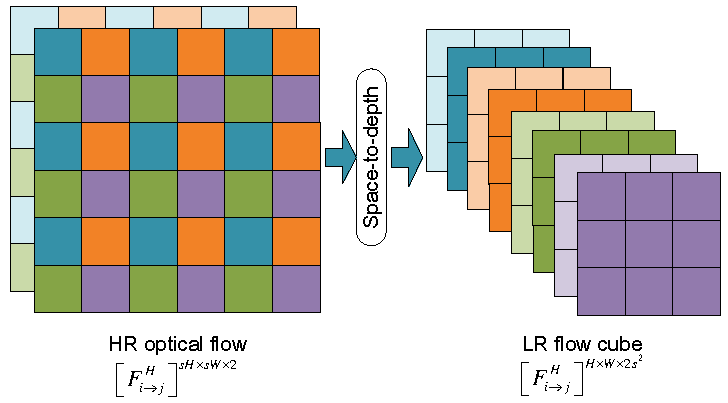
\includegraphics[clip, trim=0cm 1.4cm 0cm 0cm, height=5cm]{images/space2depth.pdf}
    \caption{SpaceToDepth module rearranges pixels from spatial dimension into channel dimension.} 
    \label{fig:space2depth}
    \end{figure}




\subsection{Fused Mobile Bottleneck Convolution (FusedMBConv)}

In the design of small and efficient networks for mobile devices a dominant and most widely used block is a so-called Mobile Bottleneck (MBConv) first proposed in \cite{howard2017_mobilenetv1} and widely used after that \cite{howard2019_searching_mobilenetv3} % TODO: add more citations here
MBConv consists of $1 \times 1$ conv $\rightarrow$ Depthwise conv $\rightarrow$ $1\times 1$ conv. As been noted in previous sections both $1\times 1$ and DepthWise convolutions could become memory-bounded if used at the beginning of the networks. The possible solution to avoid such bottleneck is to combined first two convolution together. This newly proposed block is called FusedMBConv and was first proposed in \cite{li2021_searching} and lately used in \cite{tan2021_efficientnetv2}, the Figure \ref{fig:fusedmbconv} illustrates the difference between MBConv and FusedMBConvs

\begin{figure}[h!]
    \centering
        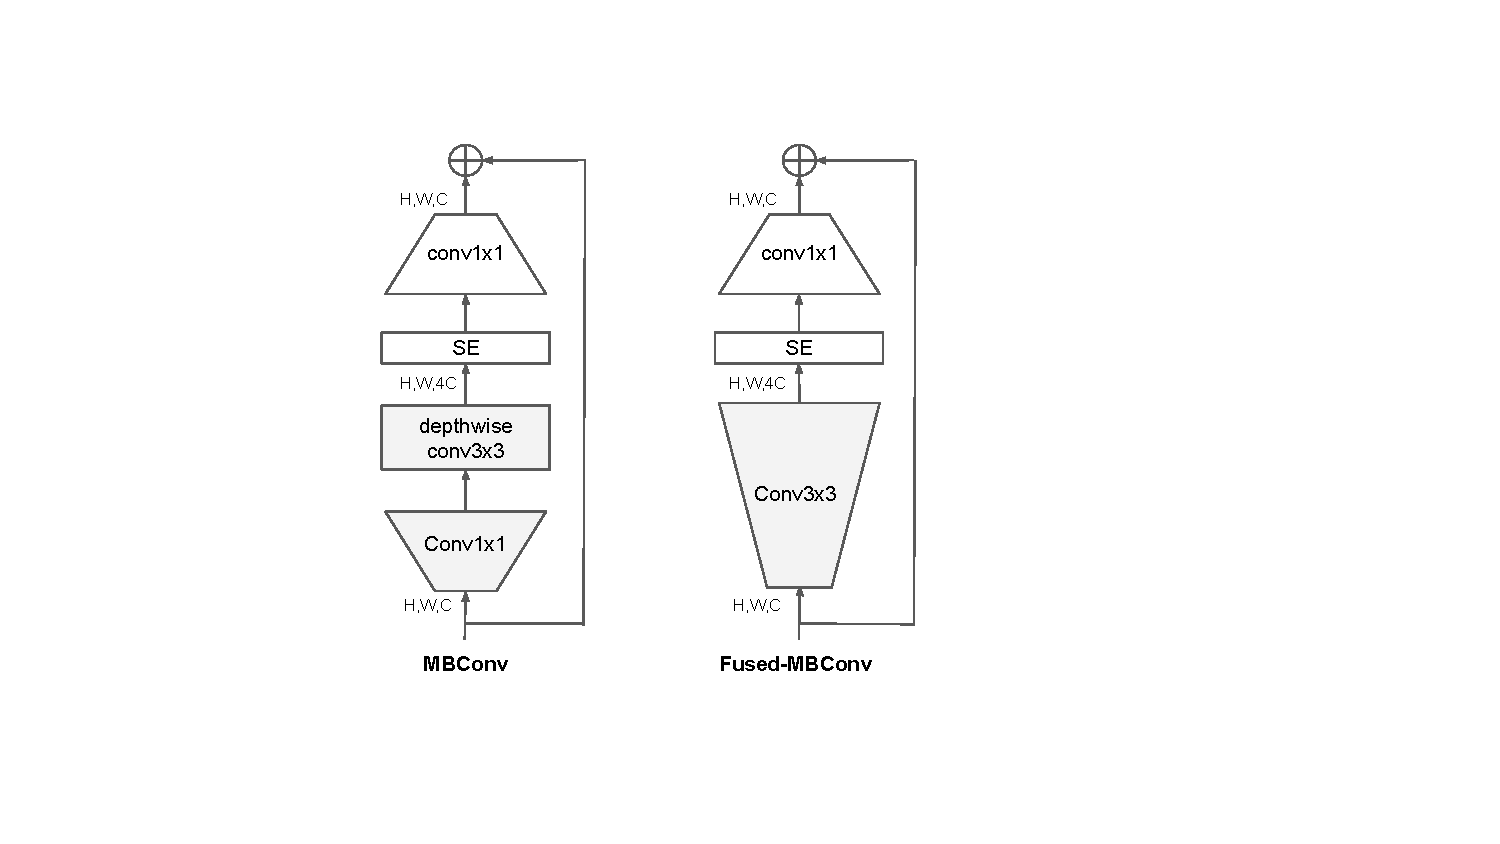
\includegraphics[clip, height=8cm]{images/fusedmbconv.pdf}
    % \caption{SpaceToDepth module rearranges pixels from spatial dimension into channel dimension.} 
    \caption{Structure of Mobile Bottleneck Convolution (MBConv) and Fused-MBConv}
    \label{fig:fusedmbconv}
    \end{figure}




%  + тут можно написать про FusedConv который есть в EffNet v2, но появился вроде в EffNetX (??) 
% кусок нагло спизжен из Searching for Fast .... нужно будет переписать. 
% еще про space2depth написано в статье \cite{ridnik2021_tresnet}


% 3.1. Efficient space-to-depth and space-to-batch
% As pointed out in Section 2, convolutions need high parallelism in all dimensions (depth, batch, and spatial) to achieve high speed on TPUs and GPUs. However, insufficient parallelism because of the small depth and batch is the usual cause of low utilization and low performance on matrix units. We augment the search space with accelerator-friendly spaceto-depth and space-to-batch ops to increase depth and batch dimensions while keeping the total tensor volume the same. For space-to-depth ops, instead of using the memorycopy-reshape based ops provided by frameworks such as TensorFlow [6] and Pytorch [42], we customize an $n \times n$ convolution with stride-n to perform the space-to-depth operation, reshaping an $H \times W \times C$ tensor to an $H / n \times W / n \times C * n^{2}$ tensor. This approach has two advantages: 1) convolutions are much preferred by TPUs and GPUs because of their high operational intensity and execution efficiency; 2) in addition to reshaping the input tensor to improve operational intensity and efficiency, the $n \times n$ convolutions can also be trained
 
% кусок из основной статье про TResNet. нужно переписать так, чтобы это не сильно пересекалось с тем, что написано в ablation про input stem
% SpaceToDepth Stem - Neural networks usually start with a stem unit - a component whose goal is to quickly reduce the input resolution. ResNet50 stem is comprised of a stride-2 conv7x7 followed by a max pooling layer [10], which reduces the input resolution by a factor of 4 (224 → 56). ResNet50-D stem design [11], for comparison, is more elaborate - the conv7x7 is replaced by three conv3x3 layers. The new ResNet50-D stem design did improve accuracy, but at a cost of lowering the training throughput - see Table 1, where the new stem design is responsible for almost all the decline in the throughput. We wanted to replace the traditional convolution-based downscaling unit by a fast and seamless layer, with little information loss as possible, and let the well-designed residual blocks do all the actual processing work. The new stem layer sole functionality should be to downscale the input resolution to match the rest of the architecture, e.g., by a factor of 4. We met these goals by using a dedicated SpaceToDepth transformation layer [33], that rearranges blocks of spatial data into depth. Notice that in contrast to [33], which mainly used SpaceToDepth in the context of isometric (single-resolution) networks, in our novel design SpaceToDepth is used as a drop-in replacement for the tradition stem unit. The SpaceToDepth layer is followed by simple convolution, to match the number of wanted channels, as can be seen in Figure 1.